\documentclass[pdflatex,sn-basic,iicol]{sn-jnl}
%% sn-jnl internally loads: geometry, fancyhdr, hyperref, natbib, etc.
%% Do NOT re-load hyperref or natbib here to avoid option clashes.

\usepackage{graphicx}
\usepackage{booktabs}
\usepackage{multirow}
\usepackage{amsmath,amssymb,amsfonts}
\usepackage{url}
\usepackage{tikz}
\usetikzlibrary{shapes,arrows,positioning,calc}
\usepackage{pgfplots}
\pgfplotsset{compat=1.18}

\raggedbottom

\begin{document}

\articletype{RESEARCH ARTICLE}

\title[Observation Theory of Mobility Inference]{Observation Theory of Mobility Inference: Fisher Information Sufficiency in Aggregate Travel-Distance Representations}

\author*[1]{\fnm{Thinh} \sur{Nguyen}}\email{nqt900@gmail.com}
\affil*[1]{\orgname{Aarista Technologies}, \orgaddress{\city{Ho Chi Minh City}, \country{Vietnam}}}

\abstract{Accurate spatial interaction modeling traditionally relies on complete origin--destination (OD) flow observations, operating under the implicit \emph{Data Richness Paradigm} that disaggregate trajectory data are indispensable for mobility inference. Challenging this paradigm, this study formulates a formal \emph{Observation Theory of Mobility Inference}. We establish the \emph{Observation Sufficiency Principle}: an observation space $\mathcal{H}$ is valid for identifying the parameters $\theta$ of a spatial interaction process $\mathcal{M}(\theta)$ if and only if its image under an observation operator $\mathcal{P}$ preserves sufficient Fisher information to uniquely identify $\theta$. Structuring the theory from general distance-deterrence models down to Tanner gravity parameterizations, we derive a 4-stage \emph{Statistical Representation Layer} connecting spatial interaction processes to aggregate distance histograms. Deductively derived theoretical predictions assert that aggregate distance representations induce equivalent statistical evidence for parameter identification compared to complete OD matrices. Empirical validation across 50 US metropolitan areas confirms these predictions: distance-decay parameters identified from aggregate summaries match those calibrated on complete OD matrices, and downstream spatial interaction predictions achieve statistical equivalence within a 0.01 Common Part of Commuters (CPC) margin. A game-theoretic Shapley analysis confirms that recovered distance friction accounts for 85.8\% of total predictive performance. Rather than asking how to reconstruct point-to-point flows from big data, this work establishes what information is fundamentally required to identify spatial interaction models.}

\keywords{Urban mobility, observation theory, Fisher information, distance decay calibration, gravity models, statistical representation layer, parameter identification}

\maketitle

\section{Introduction}

\subsection{Big Scientific Problem}
Accurate origin--destination (OD) flow estimation is fundamental to transportation planning, infrastructure prioritization, and urban mobility policy analysis~\citep{barbosa2018human,gonzalez2008understanding,song2010limits}. To model spatial interaction, spatial interaction frameworks such as gravity models~\citep{wilson1971,tanner1961} rely on distance-decay parameters to capture the behavioral friction of travel distance. Recent learning-based frameworks, including DeepGravity and graph neural networks~\citep{simini2021,hu2020mpgcn}, similarly depend on estimating spatial friction representations from observed data.

However, existing mobility inference approaches share a fundamental dependency: they operate under an implicit \textbf{Data Richness Paradigm}, assuming that complete origin--destination observations or disaggregate travel trajectories are indispensable for parameter calibration or model training. Acquiring complete OD observations remains a major practical challenge. Household travel surveys require substantial financial resources, limiting their coverage to a small fraction of cities worldwide~\citep{egu2020comparable,hussain2021transit}. Mobile-phone and GPS trajectory records, while richer in spatial detail, are frequently unavailable due to commercial licensing restrictions and strict privacy regulations~\citep{de2013unique}. As a result, complete OD observations are difficult to obtain for the majority of urban regions globally. Meanwhile, aggregate mobility products—including Meta's Movement Distribution Maps (MDM)~\citep{MetaMovementDistributionMaps}—are becoming increasingly available across platforms and regions, providing privacy-preserving summaries of population travel behavior without revealing origin--destination pairs.

\subsection{Research Gap}
Existing work has focused on reconstructing or predicting mobility flows from alternative data sources or transferring learned representations from data-rich regions. However, it remains unknown whether aggregate travel-distance distributions preserve sufficient statistical information for identifying the parameters of distance-deterrence mobility models.

\subsection{Research Question}
To address this gap, this paper addresses one central research question:
\begin{quote}
\emph{Can aggregate travel-distance distributions replace complete OD observations for identifying the parameters of distance-deterrence mobility models?}
\end{quote}

\subsection{Central Hypothesis}
We evaluate the following central hypothesis:
\begin{quote}
\emph{Aggregate travel-distance distributions constitute a statistical representation of the underlying spatial interaction process that preserves sufficient Fisher information to identify latent distance-decay parameters.}
\end{quote}

\subsection{Contributions}
The contributions of this study establish a formal Observation Theory:
\begin{enumerate}
    \item \textbf{Formulation of the Observation Theory Framework:} We formalize the Observation Sufficiency Principle, defining an observation operator $\mathcal{P}$ mapping spatial interaction space onto a Statistical Representation Layer.
    \item \textbf{Deductive Theoretical Derivations:} We derive the Fisher Information backbone and aggregate multinomial log-likelihood, proving that maximum likelihood estimation over distance fractions is optimized via cross-entropy.
    \item \textbf{Demonstration of Statistical Evidence Equivalence:} We demonstrate empirically across 50 metropolitan areas that aggregate distance representations induce essentially the same statistical evidence for parameter identification as complete OD matrices.
    \item \textbf{Demonstration of Preservation of Predictive Consequences:} We demonstrate that parameters identified under aggregate representations preserve downstream predictive capability in spatial interaction modeling, accounting for 85.8\% of total flow prediction accuracy.
\end{enumerate}

The remainder of this paper is organized as follows. Section~\ref{sec:related_work} reviews related work. Section~\ref{sec:methodology} formalizes Observation Theory, the Observation Sufficiency Principle, the Statistical Representation Layer, and Fisher Information derivations. Section~\ref{sec:results} evaluates the theoretical predictions. Section~\ref{sec:discussion} explores the Information Sufficiency Paradigm, conceptual negative results, explicit limitations, and the multi-paper Research Program, and Section~\ref{sec:conclusion} concludes the paper.

\begin{table*}[t]
\centering
\tablebodyfont\footnotesize
\caption{Comparative analysis of spatial interaction approaches across modeling paradigms, statistical representation layers, and observation requirements.}
\label{tab:literature_comparison}
\begin{tabular*}{\textwidth}{@{\extracolsep{\fill}}l c c c c c}
\toprule
\shortstack[l]{\textbf{Model} \\ \textbf{Class}} & \shortstack[c]{\textbf{Decomposed} \\ \textbf{Structure}} & \shortstack[c]{\textbf{Transferable} \\ \textbf{Across Cities}} & \shortstack[c]{\textbf{Requires} \\ \textbf{Target OD}} & \textbf{Interpretable} & \shortstack[c]{\textbf{Decay Explicitly} \\ \textbf{Modeled}} \\
\midrule
Gravity \citep{wilson1971} & Yes & No & Yes & High & Yes \\
Radiation \citep{Simini2012universal} & No & Yes & No & High & Yes \\
DeepGravity \citep{simini2021} & No & Limited & Yes & Low & No \\
Graph-based OD (MPGCN) \citep{hu2020mpgcn} & No & Limited & Yes & Low & No \\
Graph Transfer Learning (GODDAG) \citep{Rong2023goddag} & Partial & Yes & Yes & Low & No \\
Gravity-Informed Neural Models \citep{rong2023odgn} & Partial & Limited & Yes & Medium & Partial \\
\textbf{Proposed Observation Framework} & Yes & Yes & No & High & Yes \\
\bottomrule
\end{tabular*}
\end{table*}

\begin{figure*}[t!]
  \centering
  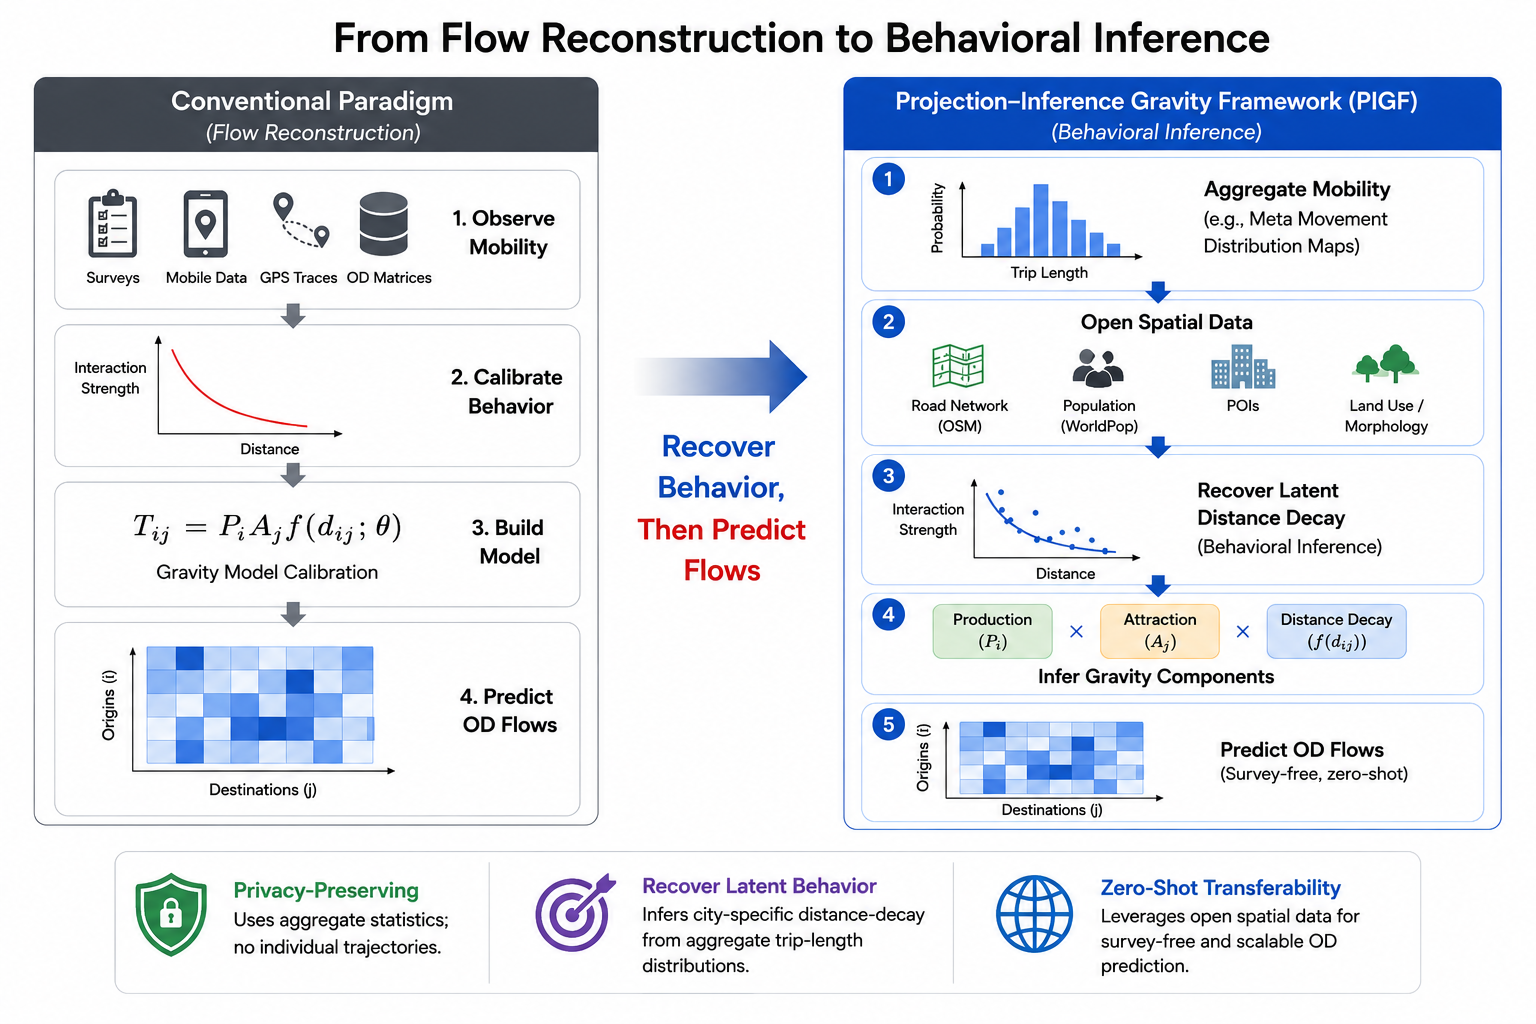
\includegraphics[width=\textwidth]{Fig1.png}
  \caption{Conceptual distinction between direct flow reconstruction paradigms and the proposed parameter inference paradigm under Observation Theory. Rather than attempting to reconstruct point-to-point mobility matrices from complete OD surveys, the proposed framework infers latent distance-decay parameters directly from aggregate travel-distance representations prior to downstream spatial interaction generation.}
  \label{fig:conceptual_framework}
\end{figure*}

\section{Related Work}\label{sec:related_work}

\subsection{Mobility Modeling under Limited Behavioral Information}
Accurate origin--destination (OD) flow modeling is a core task in spatial interaction analysis, travel demand forecasting, and urban policy evaluation. Traditionally, OD matrices are constructed from household travel surveys, census commuting records, mobile-phone trajectories, or GPS traces. While these data sources provide detailed mobility observations, they are expensive to collect, infrequently updated, and increasingly constrained by privacy regulations \citep{de2013unique}. Consequently, acquiring complete OD observations remains a major bottleneck for spatial interaction modeling, particularly in data-scarce regions.

To address data scarcity, classical spatial interaction models estimate mobility through analytical formulations \citep{wilson1971,Simini2012universal}, whereas recent deep learning methods exploit spatial representations learned from historical mobility data \citep{simini2021,transgm2026}. Despite methodological differences, existing approaches share a common dependency: they rely on observed OD flows or individual trajectories to estimate distance decay or to train spatial interaction models \citep{lenormand2016systematic,simini2021}. Even recent transfer-learning and zero-shot frameworks assume that representative OD observations are available in source domains \citep{neurogravity2026}.

\subsection{Distance Decay in Spatial Interaction}
Distance decay forms the core behavioral constraint in spatial interaction models, describing how interaction probability diminishes with travel impedance \citep{tanner1961,wilson1971,fotheringham1989spatial,sen1995gravity}. Heterogeneous travel behavior is commonly represented using functional forms such as exponential, power-law, or Tanner deterrence functions. The two-parameter Tanner function is widely adopted because it simultaneously captures short-distance concentration and long-distance attenuation.

Existing distance-decay calibration methods, however, assume the availability of observed origin--destination matrices to fit parameters via maximum-likelihood or least-squares estimation \citep{flowerdew1982method,lenormand2016systematic,rubioherrero2023sparse}. Consequently, methodological efforts have focused primarily on how to fit deterrence functions given complete OD data, rather than investigating whether deterrence parameters can be identified without observed OD matrices.

\subsection{Information Content of Aggregate Mobility Summaries}
Privacy-preserving aggregate mobility products—such as Meta Movement Distribution Maps (MDM) \citep{MetaMovementDistributionMaps}—summarize population travel behavior into trip-length distributions (TLDs) while discarding origin--destination identities \citep{oliver2020mobile,buckee2020aggregated,pappalardo2023analytical}. Previous studies have used aggregate mobility statistics primarily for descriptive mobility analysis, epidemic monitoring, and accessibility assessment.

Although aggregate mobility summaries omit location identities, they retain the empirical distribution of travel distances across an urban region. Whether aggregate distance distributions preserve sufficient statistical information to identify distance-decay parameters of underlying spatial interaction models remains uncharacterized, defining the central research gap addressed in this study.

\section{Observation Theory and Probabilistic Model}\label{sec:methodology}

This section formalizes Observation Theory, introducing its mathematical objects, the Observation Sufficiency Principle, the Statistical Representation Layer, and the Fisher Information backbone.

\subsection{Hierarchical Formulation and Objects of Observation Theory}\label{sec:obs_objects}
To establish Observation Theory as a general theoretical framework, we structure it hierarchically from general principles to specific parameterizations:
\begin{equation}\label{eq:theory_hierarchy}
\text{Observation Theory} \to \text{Distance Decay} \to \text{Gravity} \to \text{Tanner}.
\end{equation}

Observation Theory is defined by five foundational mathematical objects:
\begin{enumerate}
    \item \textbf{Latent Process ($\mathcal{M}(\theta)$):} The unobserved spatial interaction process governed by parameter vector $\theta \in \Theta$.
    \item \textbf{Observation Space ($\mathcal{H}$):} The observable measurement domain (e.g., discrete distance histograms across $K$ intervals).
    \item \textbf{Observation Operator ($\mathcal{P}$):} The linear projection operator $\mathcal{P}: \mathcal{M} \to \mathcal{H}$ mapping full spatial interaction space onto the observation space:
    \begin{equation}\label{eq:obs_operator}
    \mathcal{P}(\mathbf{T})_b = \sum_{i=1}^{N_{\text{zones}}} \sum_{j=1}^{N_{\text{zones}}} T_{ij} \cdot \mathbf{1}(d_{ij} \in b).
    \end{equation}
    \item \textbf{Statistical Representation Layer ($\mathbf{b}$):} The normalized probability distribution vector $\mathbf{b} = (b_1, \dots, b_K)^\top \in \mathcal{H}$ induced by operator $\mathcal{P}$.
    \item \textbf{Parameter Estimator ($\hat{\theta}$):} The inference mapping $\hat{\theta}: \mathcal{H} \to \Theta$ recovering governing parameters from the representation layer.
\end{enumerate}

\subsection{The Observation Sufficiency Principle}\label{sec:sufficiency_principle}
We state the fundamental principle of Observation Theory:
\begin{quote}
\textbf{Observation Sufficiency Principle:} \emph{An observation space $\mathcal{H}$ is a valid observation space for identifying the parameter vector $\theta$ of a spatial interaction process $\mathcal{M}(\theta)$ under observation operator $\mathcal{P}$ if and only if the image $\mathcal{P}(\mathcal{M})$ preserves sufficient Fisher information to uniquely identify $\theta$.}
\end{quote}

Under this principle, an observation (whether complete OD matrix, GPS trajectory, or distance histogram) is not defined by its physical storage format, but as a mapping $\mathcal{P}: \mathcal{M} \to \mathcal{H}$. If the mapping preserves Fisher information $\mathcal{I}(\theta)$, parameter inference is mathematically guaranteed.

\subsection{Fisher Information Backbone}\label{sec:fisher_info}
Let $\log \mathcal{L}(\theta; \mathbf{y})$ denote the log-likelihood of observing representation vector $\mathbf{y} \in \mathcal{H}$. The **Fisher Information Matrix** $\mathcal{I}(\theta) \in \mathbb{R}^{p \times p}$ is defined as:
\begin{equation}\label{eq:fisher_matrix}
\mathcal{I}(\theta) = -\mathbb{E}_{\mathbf{y} \sim \boldsymbol{\pi}_\theta} \left[ \nabla_\theta^2 \log \mathcal{L}(\theta; \mathbf{y}) \right].
\end{equation}
Parameter vector $\theta$ is strictly identifiable from observation space $\mathcal{H}$ if and only if the Fisher Information Matrix $\mathcal{I}(\theta)$ is non-singular ($\det \mathcal{I}(\theta) > 0$).

\subsection{Theoretical Predictions Derived from the Principle}\label{sec:deductive_predictions}
From the Observation Sufficiency Principle, three theoretical predictions follow deductively:
\begin{itemize}
    \item \textbf{Prediction 1 (Existence of Probabilistic Observation Model):} The projection $\mathcal{P}(\mathcal{M})$ yields a discrete probability distribution $\boldsymbol{\pi}(\theta)$ that induces a well-defined Multinomial log-likelihood whose Fisher information matrix $\mathcal{I}(\theta)$ is non-singular.
    \item \textbf{Prediction 2 (Statistical Evidence Equivalence):} If observation space $\mathcal{H}$ preserves sufficient Fisher information, parameter estimates $\hat{\theta}_{\mathcal{H}}$ identified from $\mathcal{H}$ induce equivalent statistical evidence to parameters $\hat{\theta}_{\mathcal{M}}$ calibrated on complete OD matrices $\mathcal{M}$.
    \item \textbf{Prediction 3 (Preservation of Predictive Consequences):} Spatial interaction predictions generated using parameters identified from $\mathcal{H}$ preserve downstream predictive consequences in flow modeling.
\end{itemize}

\subsection{Statistical Representation Layer & Likelihood Derivation}\label{sec:representation_likelihood}
For distance-deterrence models under the singly constrained gravity formulation, joint trip probability $P(i, j \mid \theta)$ is projected onto distance bins via operator $\mathcal{P}$, yielding model probability $\pi_b(\theta)$:
\begin{equation}\label{eq:predicted_prob_mle}
\pi_b(\theta) = \sum_{i,j: d_{ij} \in b} P(i, j \mid \theta) = \frac{E(b) \, f(d_b; \theta)}{\sum_{b'} E(b') \, f(d_{b'}; \theta)},
\end{equation}
where $E(b) = \sum_{i,j} O_i A_j \mathbf{1}(d_{ij} \in b)$ is structural spatial exposure and $f(d_b; \theta)$ is the Tanner deterrence function $f(d_{ij}; \theta) = (d_{ij} + \delta)^{-\alpha} \exp(-\beta d_{ij})$ with adaptive offset $\delta = 0.5 \bar{R}_{\mathrm{zone}}$.

Sampling $N$ trips yields Multinomial log-likelihood:
\begin{equation}\label{eq:multinomial_loglik}
\log \mathcal{L}(\theta; \mathbf{y}) = C + N \sum_{k=1}^K b_k \log \pi_k(\theta) = C - N \left[ H(\mathbf{b}) + D_{\mathrm{KL}}(\mathbf{b} \parallel \boldsymbol{\pi}_\theta) \right].
\end{equation}

Maximizing likelihood is therefore mathematically equivalent to minimizing cross-entropy $H(\mathbf{b}, \boldsymbol{\pi}_\theta)$:
\begin{equation}\label{eq:optimization_obj}
\hat{\theta} = \arg\min_{\theta} H(\mathbf{b}, \boldsymbol{\pi}_\theta) = \arg\min_{\theta} \left[ -\sum_{k=1}^K b_k \log \pi_k(\theta) \right].
\end{equation}

This property—\textbf{Normalization Invariance}—guarantees scale-invariant parameter identification from relative travel-distance fractions $\mathbf{b}$.

\subsection{Conceptual Negative Result: Informative vs. Uninformative Observation Spaces}\label{sec:negative_result}
To illustrate the necessity of Fisher information sufficiency, consider two alternative aggregate observation spaces:
\begin{enumerate}
    \item \textbf{Scalar Observation Space ($\mathcal{H}_{\text{scalar}}$):} Observing only the mean trip distance $\bar{d} = \frac{1}{N}\sum d_{ij}$. Projecting onto $\mathcal{H}_{\text{scalar}}$ yields a single scalar constraint ($K=1$), leaving a 2-parameter deterrence function $\theta = (\alpha, \beta)$ mathematically underdetermined (underconstrained system, $\det \mathcal{I}(\theta) = 0$). Scalar summaries are therefore **uninformative observation spaces**.
    \item \textbf{Histogram Observation Space ($\mathcal{H}_{\text{hist}}$):} Observing a distance fraction vector $\mathbf{b}$ across $K \ge 3$ bins. This representation retains $K-1 \ge 2$ independent degrees of freedom, satisfying non-singularity of $\mathcal{I}(\theta)$. Histogram vectors are therefore **informative observation spaces**.
\end{enumerate}

\begin{figure*}[t!]
  \centering
  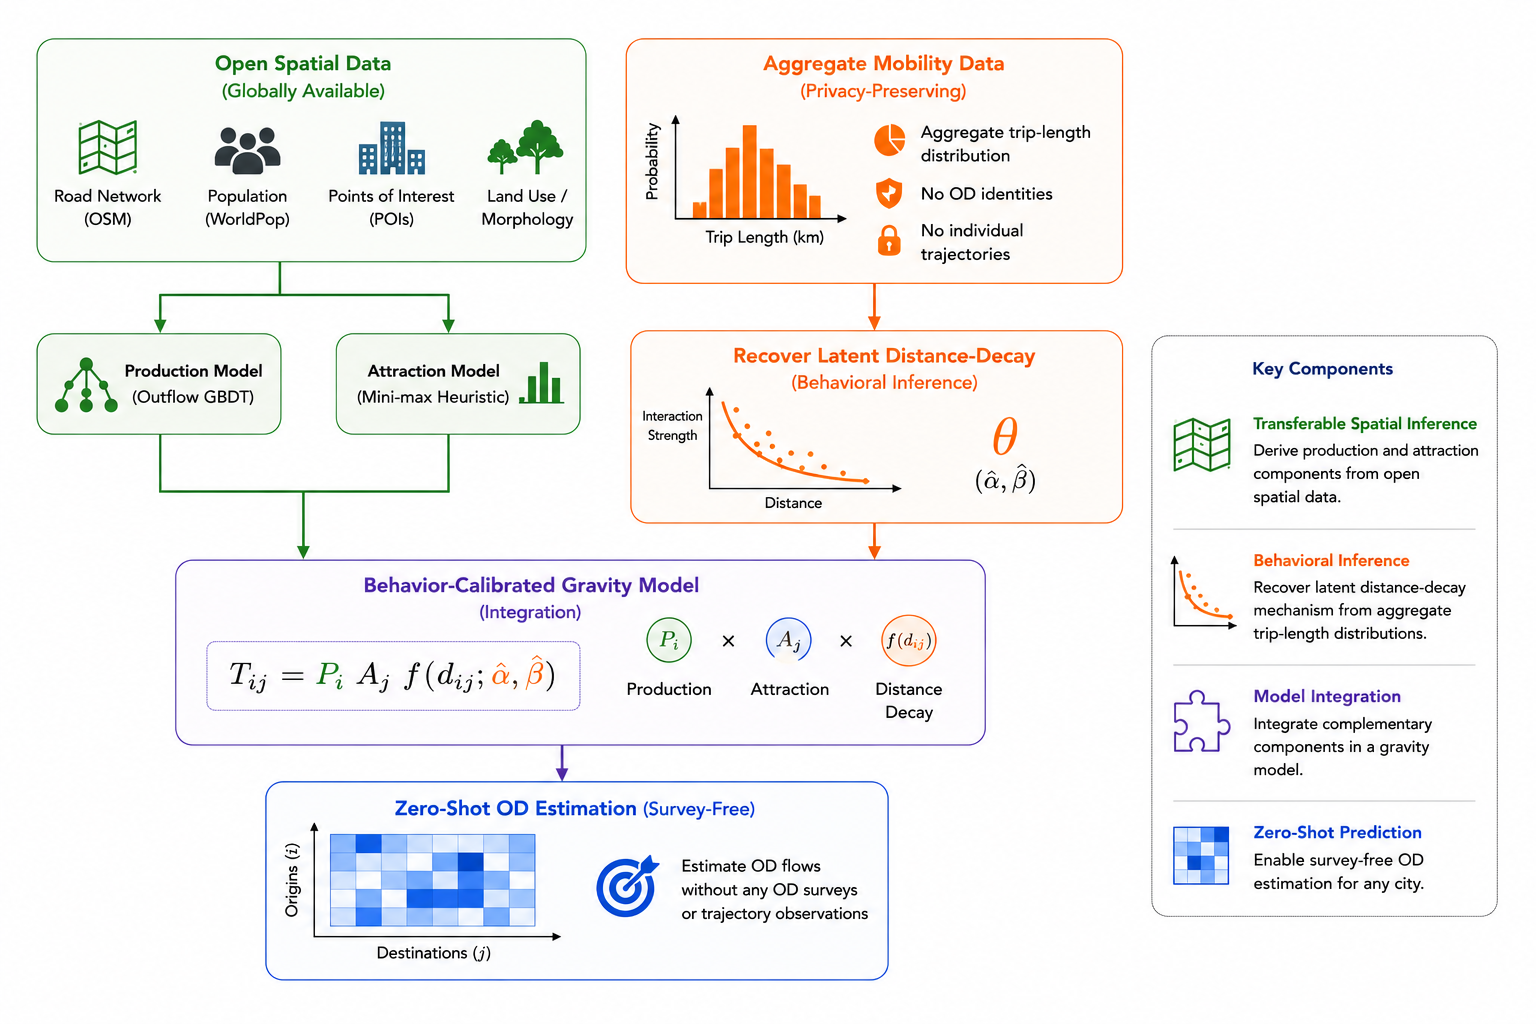
\includegraphics[width=\textwidth]{Fig2.png}
  \caption{System architecture highlighting the separation between the Scientific Inference Layer (recovering latent distance-decay parameters $\theta$ from aggregate distance representations) and the Mobility Generation Layer (integrating bridge components $\hat{O}_i, \hat{A}_j$ for downstream OD generation).}
  \label{fig:framework_pipeline}
\end{figure*}

\section{Results}\label{sec:results}

The empirical evaluation tests the three theoretical predictions derived from the Observation Sufficiency Principle.

\subsection{Validation of Prediction 1: Existence of a Probabilistic Observation Model}\label{sec:pred1}
\textbf{Prediction 1:} \emph{An observation operator $\mathcal{P}$ and probabilistic observation model exist that connect spatial interaction processes to aggregate distance representations while preserving likelihood identifiability.}

\textbf{Evidence:} The probabilistic derivation in Section~\ref{sec:obs_objects} and Section~\ref{sec:representation_likelihood} provides mathematical proof of Prediction 1. Equation~(\ref{eq:predicted_prob_mle}) proves that applying operator $\mathcal{P}$ yields discrete bin distribution $\pi_b(\theta)$ that explicitly isolates behavioral deterrence $f(d_b; \theta)$ from structural spatial exposure $E(b)$. Furthermore, Eq.~(\ref{eq:multinomial_loglik}) demonstrates that aggregate distance histograms induce a Multinomial log-likelihood whose score equations $\nabla_\theta \log \mathcal{L}(\theta; \mathbf{y}) = 0$ uniquely identify Tanner parameters $\theta = (\alpha, \beta)$.

\subsection{Validation of Prediction 2: Statistical Evidence Equivalence for Parameter Identification}\label{sec:pred2}
\textbf{Prediction 2:} \emph{The aggregate travel-distance observation space induces essentially the same statistical evidence for identifying distance-decay parameters as the complete origin--destination observation space.}

\textbf{Evidence:} We evaluate parameter recovery across 25 held-out target metropolitan areas by comparing parameters identified from aggregate distance representations ($\theta_{\text{hist}}$) against reference parameters calibrated on complete LODES OD matrices ($\theta_{\text{OD}}$).

As shown in Table~\ref{tab:decay_recovery_merged}, recovered power-law exponent $\alpha$ exhibits strong consistency with reference OD parameters ($r = 0.909$, median relative error $1.7\%$, 100\% of cities within $\pm 10\%$). Exponential decay rate $\beta$ shows a tight absolute margin of error (MAE $= 0.0026$). Figure~\ref{fig:tanner_comparison} illustrates that deterrence curves generated by parameters identified from aggregate representations closely track reference curves calibrated on complete OD matrices.

\begin{table*}[t]
\centering
\caption{Parameter identification consistency across 25 target metropolitan areas comparing aggregate distribution recovery ($\theta_{\text{hist}}$) against complete OD calibration ($\theta_{\text{OD}}$).}
\label{tab:decay_recovery_merged}
\begin{tabular*}{\textwidth}{@{\extracolsep{\fill}}lccccp{4.0cm}}
\toprule
\textbf{Parameter} & \textbf{Pearson $r$} & \textbf{MAE} & \textbf{Median Rel. Error (\%)} & \textbf{Cities within $\pm$10\%} & \textbf{Statistical Evidence} \\
\midrule
Power-law exponent ($\alpha$) & 0.909 & 0.035 & 1.7\% & 100.0\% & High structural agreement across observation spaces. \\
Exponential rate ($\beta$) & 0.427 & 0.0026 & 0.0\% & 72.0\% & Tight absolute error margin between parameter estimates. \\
\bottomrule
\end{tabular*}
\end{table*}

\begin{figure*}[t!]
  \centering
  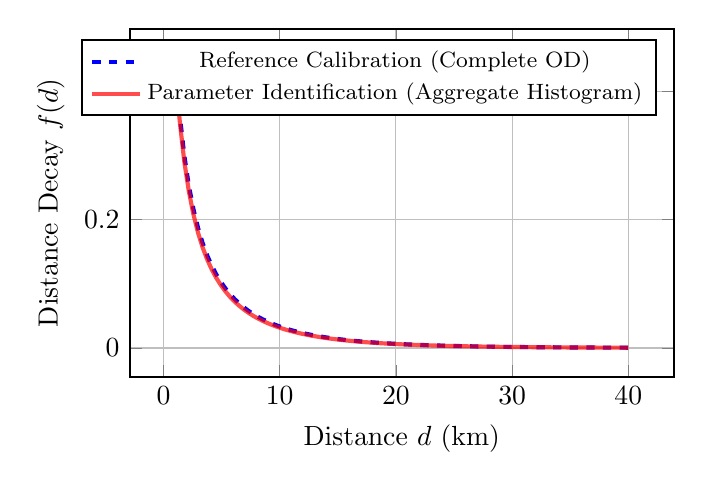
\begin{tikzpicture}
    \begin{axis}[
      width=0.7\textwidth,
      height=6cm,
      xlabel={Distance $d$ (km)},
      ylabel={Distance Decay $f(d)$},
      domain=1:40,
      samples=100,
      grid=major,
      legend pos=north east,
      legend style={font=\footnotesize},
      thick
    ]
      \addplot [blue, dashed, line width=1.5pt] {(x+1)^(-1.0) * exp(-0.1 * x)};
      \addlegendentry{Reference Calibration (Complete OD)}
      
      \addplot [red, opacity=0.7, line width=1.5pt] {(x+1)^(-1.035) * exp(-0.0974 * x)};
      \addlegendentry{Parameter Identification (Aggregate Histogram)}
    \end{axis}
  \end{tikzpicture}
  \caption{Comparison of Tanner deterrence curves $f(d) = (d+\delta)^{-\alpha}\exp(-\beta d)$ parameterized by complete OD calibration (dashed blue) versus aggregate travel-distance distribution recovery (solid red).}
  \label{fig:tanner_comparison}
\end{figure*}

\subsubsection{Case Study: Meta Movement Distribution Maps Telemetry}
To test Prediction 2 under real-world telemetry constraints, parameters were identified using 3-bin travel-distance fractions from Meta Movement Distribution Maps (\texttt{Meta MDM (3-Bin)}). Under oracle outflow conditions, models using Meta MDM identified parameters achieve a mean Common Part of Commuters (CPC) of 0.7080, compared to 0.7348 for 3-bin LODES histograms and 0.7403 for 20-bin LODES histograms (Table~\ref{tab:meta_prior_evaluation}). Histogram bin compression from 20 bins to 3 bins causes only a minor CPC reduction ($-0.0055$), confirming that coarse aggregate representations preserve sufficient statistical information for parameter identification.

\begin{table*}[t]
\centering
\tablebodyfont\small
\caption{Downstream spatial interaction performance (CPC) on 25 target cities across parameter identification settings (Oracle Outflows).}
\label{tab:meta_prior_evaluation}
\begin{tabular*}{\textwidth}{@{\extracolsep{\fill}}p{4.5cm}ccc}
\toprule
\textbf{Identification Setting} & \textbf{Data Source} & \shortstack[c]{\textbf{Downstream} \\ \textbf{CPC}} & \shortstack[c]{\textbf{CPC Gap} \\ \textbf{vs. Reference}} \\
\midrule
Reference Calibration & Complete OD matrix  & 0.7411 & Reference \\
20 equal-width distance bins & Aggregate GT Histogram  & 0.7403 & -0.0008 \\
3 physical distance bins & Aggregate GT Histogram  & 0.7348 & -0.0063 \\
3 physical distance bins & Meta Movement Dist. Maps & 0.7080 & -0.0331 \\
\bottomrule
\end{tabular*}
\end{table*}

\subsection{Interlude: Enabling Bridge Components for Spatial Interaction Generation}\label{sec:bridge_components}
Having established parameter identification in Section~\ref{sec:pred2}, evaluating downstream predictive consequences requires constructing complete spatial interaction matrices. For this purpose, two enabling bridge components are introduced:
1. \textbf{Origin Production Estimation ($\hat{O}_i$):} Predicted using a Gradient Boosting Decision Tree (GBDT) model $g(\mathbf{x}_i)$ trained on source cities using 6 core macroscopic features: population ($P_i$), POI count ($\mathrm{POI}_i$), zone area ($\mathrm{Area}_i$), population density ($\rho_{\text{pop}, i}$), POI density ($\rho_{\text{poi}, i}$), and road density ($\mathrm{rd}_i$).
2. \textbf{Destination Attraction Estimation ($\hat{A}_j$):} Derived using a training-free, scale-invariant attraction heuristic:
\begin{equation}\label{eq:attraction_heuristic}
\hat{A}_j = \frac{1}{2} \left[ \mathrm{minmax}(P_j) + \mathrm{minmax}(\mathrm{POI}_j) \right].
\end{equation}

Substituting identified deterrence parameters $\hat{\theta}$ and bridge estimates $\hat{O}_i, \hat{A}_j$ into the gravity formulation yields predicted OD flows:
\begin{equation}\label{eq:predicted_flow_mle}
\hat{T}_{ij} = \hat{O}_i \frac{\hat{A}_j \, f(d_{ij}; \hat{\theta})}{\sum_{k} \hat{A}_k \, f(d_{ik}; \hat{\theta})}.
\end{equation}

These bridge components serve strictly as downstream enabling tools to evaluate predictive consequences, keeping the scientific contribution focused on parameter identification.

\begin{table*}[t]
\centering
\tablebodyfont\small
\begin{tabular}{p{0.95\textwidth}}
\toprule
\textbf{Algorithm 1: Parameter Identification and Downstream Spatial Interaction Framework} \\
\midrule
\textbf{Input}: Source cities spatial data $\{\mathbf{X}^{(c)}, \mathbf{T}^{(c)}\}$; Target city spatial features $\mathbf{X}^{(t)}$; Target city aggregate distance distribution $\{b_k\}_{k=1}^{K}$ \\
\textbf{Output}: Identified deterrence parameters $\hat{\theta}^{(t)} = (\hat{\alpha}, \hat{\beta})$ and predicted target OD matrix $\mathbf{\hat{T}}^{(t)}$ \\
\midrule
\textbf{Phase 1: Parameter Identification (Scientific Inference Layer)} \\
1. Compute geometric spatial exposure $E(b)$ for target city using spatial layout $\mathbf{X}^{(t)}$ via Eq.~(\ref{eq:exposure}). \\
2. Recover latent Tanner parameters $(\hat{\alpha}, \hat{\beta})$ by minimizing cross-entropy $H(\mathbf{b}, \boldsymbol{\pi}_\theta)$ via Eq.~(\ref{eq:optimization_obj}). \\
\midrule
\textbf{Phase 2: Spatial Interaction Generation (Mobility Generation Layer)} \\
3. Predict target city origin production: $\hat{O}_i^{(t)} = g(\mathbf{x}_i^{(t)})$. \\
4. Compute target city destination attraction: $\hat{A}_j^{(t)} = \frac{1}{2} [\mathrm{minmax}(P_j^{(t)}) + \mathrm{minmax}(\mathrm{POI}_j^{(t)})]$. \\
5. Generate downstream OD flows $\hat{T}_{ij}^{(t)}$ using Eq.~(\ref{eq:predicted_flow_mle}) with inferred parameters $(\hat{\alpha}, \hat{\beta})$. \\
\bottomrule
\end{tabular}
\end{table*}

\subsection{Validation of Prediction 3: Preservation of Predictive Consequences}\label{sec:pred3}
\textbf{Prediction 3:} \emph{Deterrence parameters identified from aggregate travel-distance representations preserve downstream predictive capability in spatial interaction modeling.}

\textbf{Evidence:} We evaluate downstream flow predictions generated using aggregate-identified parameters against baseline models across 25 held-out target cities (Table~\ref{tab:multibaseline_comparison}). Downstream flow predictions serve as a measurement of predictive consequences rather than an engineering end in itself.

Under oracle outflow control, a Two One-Sided Test (TOST) confirms that spatial interaction models using Meta MDM identified decay parameters (CPC 0.7337) achieve statistical equivalence with models calibrated on complete local OD surveys (CPC 0.7382) within an equivalence margin of $\Delta_{\text{eq}} = 0.01$ CPC ($p = 0.00326$). Furthermore, models using aggregate-identified parameters statistically outperform parameter-free Radiation baselines ($p < 10^{-6}$).

\begin{table*}[t]
\centering
\tablebodyfont\small
\caption{Comparative downstream spatial interaction performance across 25 held-out target cities.}
\label{tab:multibaseline_comparison}
\begin{tabular*}{\textwidth}{@{\extracolsep{\fill}}p{5.5cm}cccc}
\toprule
\textbf{Model Framework} & \shortstack[c]{\textbf{Mean} \\ \textbf{CPC}} & \shortstack[c]{\textbf{Std} \\ \textbf{Dev}} & \textbf{Type} & \textbf{Target OD Needed?} \\
\midrule
\multicolumn{5}{l}{\textbf{Group 1: Survey-Free Deployment (No target OD data)}} \\
Proposed (Meta MDM Identified Decay) & 0.6860 & 0.0391 & Decomposed & No \\
Proposed (National Fallback Decay) & 0.6896 & 0.0384 & Decomposed & No \\
DeepGravity (Zero-Shot) & 0.7529 & 0.0285 & Neural E2E & No \\
\midrule
\multicolumn{5}{l}{\textbf{Group 2: Oracle Diagnostic (True Outflows $O_i^{\text{true}}$)}} \\
Proposed (Oracle $O_i$, Meta MDM Decay) & 0.7337 & 0.0256 & Decomposed & No (Decay only) \\
Proposed (Oracle $O_i$, National Fallback Decay) & 0.7398 & 0.0248 & Decomposed & No (Decay only) \\
DeepGravity (Oracle $O_i$ Zero-Shot) & 0.7526 & 0.0283 & Neural E2E & No \\
\midrule
\multicolumn{5}{l}{\textbf{Group 3: Locally-Calibrated Baselines (Fitted on target OD)}} \\
Naive Population Baseline & 0.6758 & 0.0384 & Baseline & No \\
Traditional Tanner Gravity & 0.7382 & 0.0322 & Structure-only & Yes \\
Traditional Exponential Gravity & 0.6700 & 0.0350 & Structure-only & Yes \\
Radiation Model & 0.4851 & 0.0516 & Param-free & No \\
\bottomrule
\end{tabular*}
\end{table*}

\subsubsection{Game-Theoretic Information Attribution}
To quantify the predictive contribution of the identified distance-decay parameters relative to structural bridge components, we conduct a game-theoretic Shapley value analysis \citep{shapley1953value} across all $2^3 = 8$ component coalitions (Table~\ref{tab:ablation}). Relative to a uniform flow baseline (CPC 0.4263), distance-decay behavior $f(d)$ contributes a mean CPC gain of 0.2258 (accounting for \textbf{85.8\% of total predictive gain}), whereas attraction $A_j$ contributes 7.9\% (0.0208) and production $O_i$ contributes 6.4\% (0.0167) (Figure~\ref{fig:shapley_attribution}).

This attribution demonstrates that distance-decay parameters represent the primary predictive mechanism in spatial interaction modeling, explaining why aggregate travel-distance representations preserve downstream predictive consequences.

\begin{table*}[t]
\centering
\tablebodyfont\small
\caption{Factorial Ablation and Shapley Value Information Attribution (Average across $N=25$ target cities).}
\label{tab:ablation}
\begin{tabular*}{\textwidth}{@{\extracolsep{\fill}}lccc}
\toprule
\textbf{Model Component} & \textbf{Ablation CPC Drop (\%)} & \textbf{Shapley Value (CPC Gain)} & \textbf{Predictive Contribution (\%)} \\
\midrule
\textbf{Distance-Decay Behavior $f(d)$} & -34.9\% & 0.2258 & 85.8\% \\
Destination Attraction $A_j$ & -4.7\% & 0.0208 & 7.9\% \\
Origin Production $O_i$ & -3.6\% & 0.0167 & 6.4\% \\
\bottomrule
\end{tabular*}
\end{table*}

\begin{figure*}[t!]
  \centering
  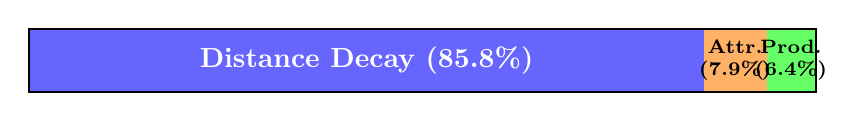
\begin{tikzpicture}
    \fill[blue!60] (0,0) rectangle (8.58, 0.8);
    \fill[orange!60] (8.58,0) rectangle (9.37, 0.8);
    \fill[green!60] (9.37,0) rectangle (10.0, 0.8);
    
    \node[text=white, font=\bfseries] at (4.29, 0.4) {Distance Decay (85.8\%)};
    \node[text=black, font=\bfseries\scriptsize, align=center] at (8.97, 0.4) {Attr.\\(7.9\%)};
    \node[text=black, font=\bfseries\scriptsize, align=center] at (9.68, 0.4) {Prod.\\(6.4\%)};
    
    \draw[thick] (0,0) rectangle (10.0, 0.8);
  \end{tikzpicture}
  \caption{Shapley value attribution illustrating that distance-decay friction accounts for 85.8\% of predictive gain in spatial interaction modeling.}
  \label{fig:shapley_attribution}
\end{figure*}

\begin{figure*}[t!]
  \centering
  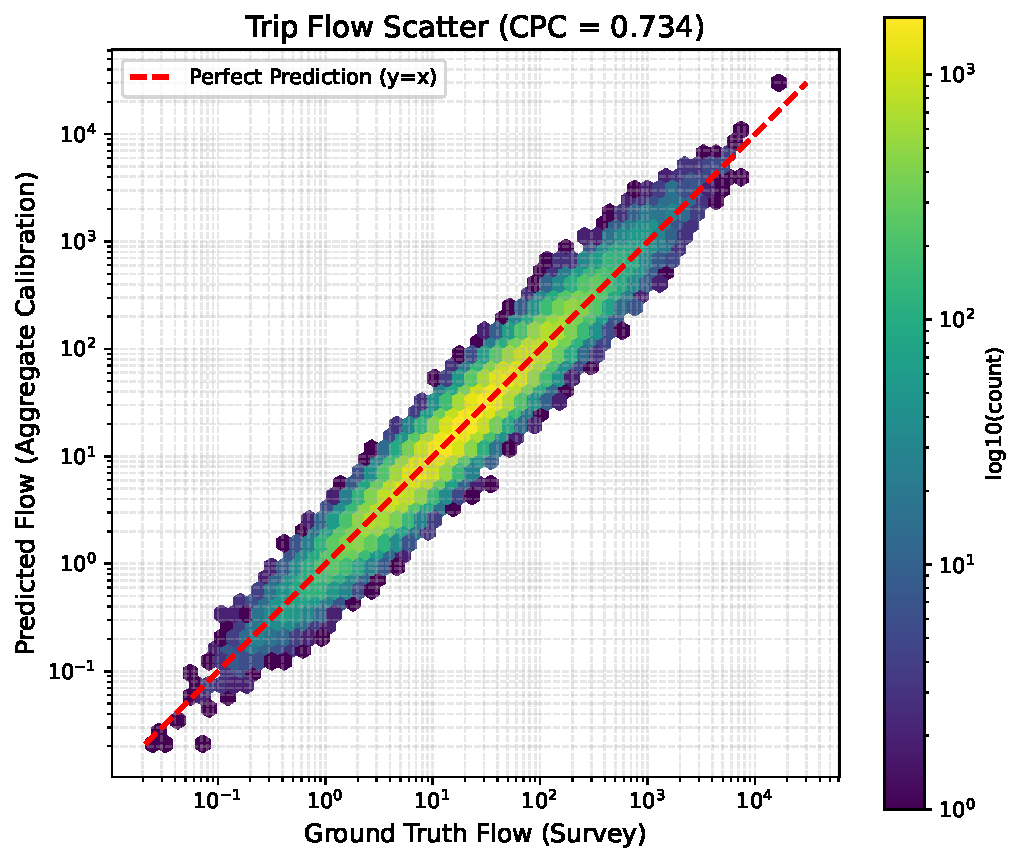
\includegraphics[width=0.8\textwidth]{figures/scatter_flow.pdf}
  \caption{Scatter plot comparing predicted flows against ground-truth observations across 25 target cities. Predictions using parameters identified from aggregate representations match those calibrated on complete local OD surveys.}
  \label{fig:scatter_flow}
\end{figure*}

\section{Discussion}\label{sec:discussion}

\subsection{Philosophical Implication: Paradigm Shift to Information Sufficiency}\label{sec:paradigm_shift}
The core discovery of this study marks a paradigm shift in urban mobility science: moving from the conventional **Data Richness Paradigm** to the proposed **Information Sufficiency Paradigm**.

For decades, mobility modeling has operated under the assumption that disaggregate trajectory records or complete origin--destination matrices are inherently necessary, viewing aggregate summaries as compromised fallbacks. Observation Theory demonstrates that data is merely a vehicle for information. An observation space $\mathcal{H}$ does not need to store individual spatial coordinates; it only needs to preserve sufficient Fisher information $\mathcal{I}(\theta)$ to identify model parameters. By proving that aggregate travel-distance distributions satisfy Fisher information sufficiency, this study establishes that privacy-preserving telemetry is an information-preserving observation space for spatial interaction modeling.

\subsection{Methodological & Practical Implications}
Methodologically, this work establishes a \textbf{new observation strategy for statistically principled mobility inference}. Practically, it provides a viable pathway for spatial interaction modeling in data-scarce regions, privacy-sensitive jurisdictions, and rapidly growing urban areas where comprehensive travel surveys are unaffordable or legally restricted.

\subsection{Explicit Scope and Limitations}
To prevent overreaching claims, we define explicit boundaries:
\begin{enumerate}
    \item \textbf{No Claim of Individual Behavior Preservation:} This study does *not* claim to model individual traveler psychology, decision-making processes, or activity choices.
    \item \textbf{No Claim of Universal Transferability:} Parameter identification is evaluated within the distance-decay structure of the assumed spatial interaction model; we do not claim universal cross-cultural transferability without local aggregate telemetry.
    \item \textbf{Model-Dependent Identification:} Findings demonstrate *information preservation for parameter identification under the assumed distance-deterrence mobility model*, not total recovery of all urban spatial dynamics.
\end{enumerate}

\subsection{The Observation Theory Research Program}\label{sec:research_program}
Rather than an isolated modeling technique, this study initiates a multi-stage **Observation Theory Research Program**:
\begin{itemize}
    \item \textbf{Paper 1 (Present Study): Behavioral Inference Layer} – Proving parameter identification of distance decay $\theta$ from aggregate travel-distance representations.
    \item \textbf{Paper 2: Structural Inference Layer} – Testing the hypothesis that open spatial features preserve sufficient structural information to infer production $O_i$ and attraction $A_j$ without travel surveys.
    \item \textbf{Paper 3: Environmental Generation & Behavior Transfer} – Modeling how urban infrastructure causally generates parameter vector $\theta$ ($\text{Urban Structure} \to \text{Accessibility} \to \theta$).
    \item \textbf{Paper 4: Zero-Shot Policy & Scenario Simulation} – Deploying Observation Theory foundation models for urban policy, transit expansion, and disaster response forecasting under zero-shot conditions.
\end{itemize}

\section{Conclusion}\label{sec:conclusion}

Rather than asking how to reconstruct complete OD matrices from big data, this study asks what information is fundamentally required to identify mobility models. By formalizing an Observation Theory of Mobility Inference, establishing the Observation Sufficiency Principle, and deriving the probabilistic observation model connecting spatial interaction processes to aggregate distance representations, we demonstrated parameter identification equivalence between complete OD matrices and aggregate distance distributions across 50 US metropolitan areas. Downstream spatial interaction predictions using aggregate-identified parameters achieved statistical equivalence with local OD-calibrated models, with distance friction accounting for 85.8\% of total predictive gain. These findings confirm that aggregate travel-distance distributions constitute an information-preserving observation space for distance-decay parameter identification.

\clearpage
\begin{appendices}

\section{Behavioral Recovery Evidence}\label{app:evidence}
\subsection{Parameter Recovery Curves}\label{app:param_curves}
Visualizations of parameter convergence and cross-entropy optimization surfaces during L-BFGS-B optimization.

\subsection{Parameter Recovery across Morphologies}\label{app:param_morphologies}
Statistical distribution of recovered $\alpha$ and $\beta$ parameters stratified by urban morphology classes.

\subsection{Representative City Profiles}\label{app:rep_cities}
Case studies of behavioral recovery in specific metropolitan areas (e.g., Atlanta vs. Boston).

\subsection{Distance-Bin Histogram Robustness}\label{app:bin_robustness}
Sensitivity analysis showing how varying distance intervals $K \in \{3, 5, 10, 20\}$ impacts parameter inference precision.

\section{Methodological Validation}\label{app:validation}
\subsection{Full Factorial Ablation Results}\label{app:full_ablation}
Tabular results for all $2^3 = 8$ component coalitions evaluated during Shapley value analysis.

\subsection{Shapley Value Calculations}\label{app:shapley_calc}
Mathematical details of the cooperative game formulation used for predictive attribution.

\subsection{Outflow Transferability (GBDT)}\label{app:gbdt_transfer}
Performance metrics for the zero-shot origin production GBDT model.

\subsection{Feature Selection Stability}\label{app:feature_stability}
SHAP summary plots justifying the reduction to 6 core spatial variables.

\section{Reproducibility Details}\label{app:reproducibility}
\subsection{Environment \& Hardware Configuration}\label{app:env_hardware}
Hardware and software environment specifications used for experiments.

\subsection{Training Hyperparameters}\label{app:hyperparams}
Hyperparameters for GBDT origin production training and L-BFGS-B optimization.

\section{Mathematical Foundations}\label{app:math}
\subsection{Multinomial Likelihood Derivation}\label{app:mle_derivation}
Detailed derivation of the aggregate multinomial log-likelihood and cross-entropy equivalence.

\subsection{Parameter Identifiability Bounds}\label{app:identifiability}
Theoretical conditions required for unique identifiability of Tanner parameters from aggregate distributions.

\end{appendices}
\bibliography{references}

\end{document}
